\documentclass[tikz, border=1cm]{standalone}
\usetikzlibrary{shapes}
\usepackage{tikz-3dplot}
\usepackage{fp}

\definecolor{tappo}{RGB}{148,154,110}
\definecolor{lightblue}{RGB}{155,210,220}



\newcommand{\newcolumn}[1]{
  \node at (24.1, #1) [cylinder, draw, shape border rotate=180, minimum height=12mm,
    minimum width=14mm, cylinder uses custom fill, cylinder body
  fill=gray!25, cylinder end fill=gray!50]{};  
  
  \node at (20.5, #1) [cylinder, draw, shape border rotate=180, minimum height=6.4cm,
  minimum width=10mm, cylinder uses custom fill, cylinder body
  fill=gray!25, cylinder end fill=gray!50]{};

  \node at (17.1, #1) [cylinder, draw, shape border rotate=180, minimum height=12mm,
    minimum width=14mm, cylinder uses custom fill, cylinder body
  fill=gray!25, cylinder end fill=gray!50]{};}

\newcommand{\singlecircle}[3]{
  \pgfmathparse{#2 > 23.5 ? 1 : 0}
  \ifthenelse{\pgfmathresult = 0} 
  {\filldraw[color=#1!60, fill=#1!45, very thick, fill opacity=0.5](#2, #3) circle (0.1);}
  {}
}

\newcommand{\circles}[2]{
  \singlecircle{black}{17.7+2.0*#2}{#1+0.20}
  \singlecircle{white}{17.9+#2}{#1+0.35}
  \singlecircle{gray}{17.8+1.5*#2}{#1+0.30}
    
  \singlecircle{gray}{18.1+1.5*#2}{#1+0.15}
  \singlecircle{black}{17.8+2.0*#2}{#1-0.15}
  \singlecircle{white}{18.0+#2}{#1+0.05}
  
  \singlecircle{white}{18.2+#2}{#1+0.10}
  \singlecircle{black}{18.1+2.0*#2}{#1+0.15}  
  \singlecircle{gray}{18.3+1.5*#2}{#1-0.25}
  
  \singlecircle{gray}{17.7+1.5*#2}{#1-0.07}
  \singlecircle{black}{18.2+2.0*#2}{#1-0.10}  
  \singlecircle{white}{18.4+#2}{#1-0.20}
}

\begin{document}

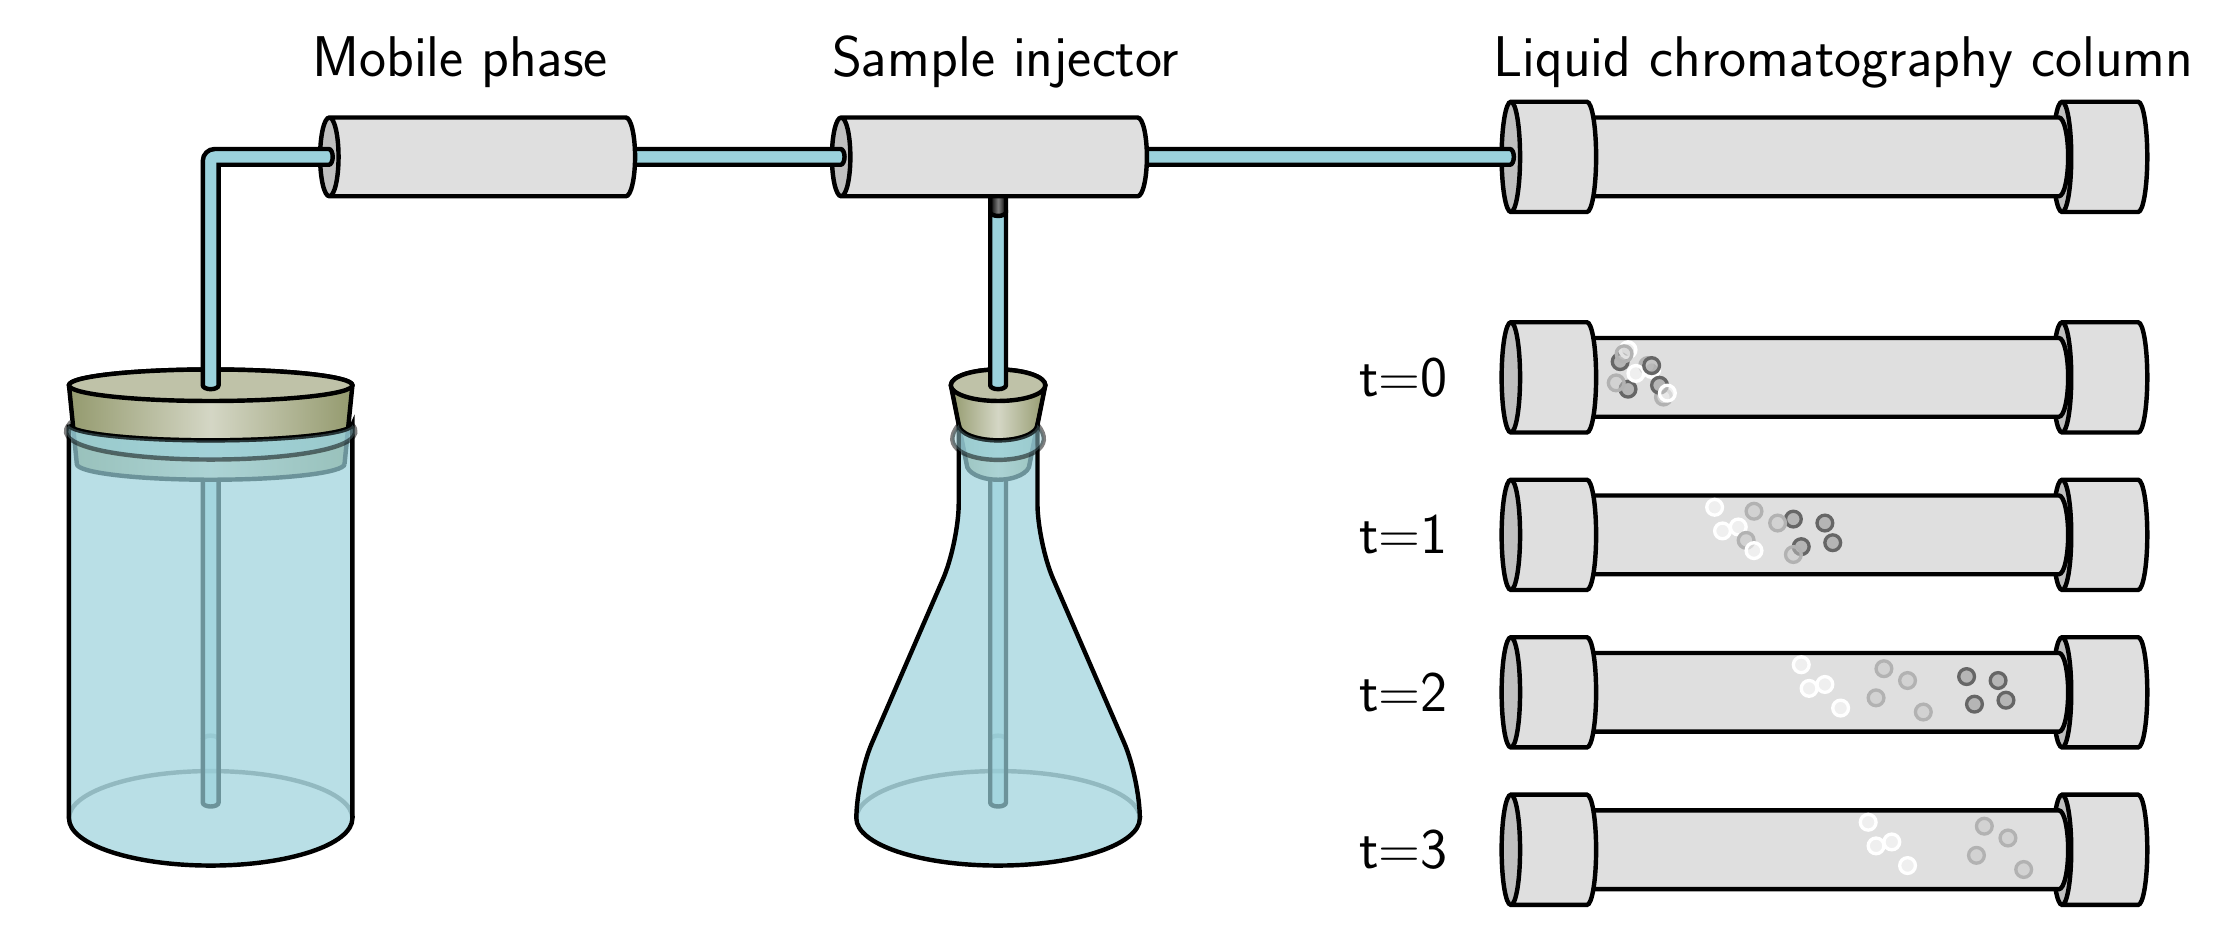
\begin{tikzpicture}[ultra thick, z={(-3mm, 4mm)}]
\newcommand{\mainscale}{1.2}

\tikzset{ mystyle/.style={draw, rotate=180, minimum height=8cm,
    minimum width=20mm, cylinder uses custom fill, cylinder body
    fill=gray!25, cylinder end fill=gray!50},
  font={\fontsize{20pt}{12}\sffamily},
  grid/.style={gray,very thin,opacity=1}
}

\begin{scope}[xshift=-12cm, yshift=0cm]

  \newcolumn{1.4}
  \node[label=right:{Liquid chromatography column}] (n1) at (16.0, 2.6) {};

  \newcolumn{-1.4}
  \node[label=left:{t=0}] (n1) at (16.0, -1.4) {};
  \circles{-1.4}{0.1}
  
  \newcolumn{-3.4}
  \node[label=left:{t=1}] (n1) at (16.0, -3.4) {};
  \circles{-3.4}{1.2}
  
  \newcolumn{-5.4}
  \node[label=left:{t=2}] (n1) at (16.0, -5.4) {};
  \circles{-5.4}{2.3}

  \newcolumn{-7.4}
  \node[label=left:{t=3}] (n1) at (16.0, -7.4) {};
  \circles{-7.4}{3.15}
  
  \draw[fill=lightblue] (10, 1.5) -- (16.5, 1.5) arc (90:-90: .5mm and 1mm) -- (10, 1.3) -- cycle;
  
  \node at (10, 1.4) [cylinder, draw, shape border rotate=180, minimum height=4cm,
  minimum width=10mm, cylinder uses custom fill, cylinder body
  fill=gray!25, cylinder end fill=gray!50,  arrowstyle/.style = {->, smooth, samples=200}]{};  
  \node[label=right:{Sample injector}] (n1) at (7.6, 2.6) {};

  \draw[fill=lightblue] (5, 1.5) -- (8, 1.5) arc (90:-90: .5mm and 1mm) -- (5, 1.3) -- cycle;
  
  \node at (3.5, 1.4) [cylinder, draw, shape border rotate=180, minimum height=4cm,
  minimum width=10mm, cylinder uses custom fill, cylinder body
  fill=gray!25, cylinder end fill=gray!50,  arrowstyle/.style = {->, smooth, samples=200}]{};  
  \node[label=right:{Mobile phase}] (n1) at (1.0, 2.6) {};

\end{scope}


% Mobile phase
\begin{scope}[xshift=-12cm, yshift=-7cm]

  % Straw
  \draw[gray] (-1.8, 0.0) arc (180:0:1.8cm and 6mm);
  \draw[gray] (0.1,1.0) arc (0:180:1mm and .5mm);
  \draw[fill=lightblue, fill opacity=.7] (.1, 4.8) -- (.1, 0.2) arc (360:180:1mm and .5mm) -- (-.1, 4.8);

  % Cork
  \draw[right color=tappo, left color=tappo, middle color=tappo!40] (1.7,4.5) --
  (1.8,5.5) arc (0:180:18mm and 2mm) --
  (-1.7, 4.5) arc (180:360:17mm and 2mm);
  \draw[fill=tappo!60] (0, 5.5) ellipse (18mm and 2mm);

  % Straw above bottle
  \fill[black] (0,5.5) ellipse (1mm and .5mm);
  \draw[fill=lightblue] (0.1, 8.3) -- (0.1, 5.5) arc (360:180:1mm and .5mm)[rounded corners=1.5mm] --
  (-0.1, 8.5) -- (1, 8.5)[sharp corners] -- (1.5, 8.5) arc (90:-90: .5mm and 1mm) -- cycle;

  % Bottle
  \draw[fill=lightblue,rounded corners=5mm, fill opacity=.7]
  (-1.8, 5.0) --
  (-1.8, 0.5) [sharp corners] --
  (-1.8, 0.0) arc (180:360:1.8cm and 6mm) [rounded corners=5mm]--
  (1.8, 0.5) --
  (1.8, 3.5) [sharp corners]--
  (1.8, 5.0) arc (360:180:18mm and 2mm);
  \draw[fill=lightblue, opacity=.5] (1.8,5) to[out=-50,in=230, looseness=0.55] (-1.8,5) arc (180:360:18mm and 2mm);
\end{scope}

% Sample
\begin{scope}[xshift=-2cm, yshift=-7cm]
  % Straw in bottle
  \draw[gray] (-1.8,0) arc (180:0:1.8cm and 6mm);
  \draw[gray] (.1,1) arc (0:180:1mm and .5mm);
  \draw[fill=lightblue, fill opacity=.7] (.1, 4.8) -- (.1, 0.2) arc (360:180:1mm and .5mm) -- (-.1, 4.8);

  % Cork
  \draw[right color=tappo, left color=tappo, middle color=tappo!40] (.4,4.5) -- (.6,5.5) arc (0:180:6mm and 2mm) -- (-.4,4.5) arc (180:360:4mm and 2mm);
  \draw[fill=tappo!60] (0, 5.5) ellipse (6mm and 2mm);

  % Straw above bottle
  \fill[black] (0,5.5) ellipse (1mm and .5mm);
  \draw[fill=lightblue] (0.1, 7.7) -- (.1,5.5) arc (360:180:1mm and .5mm) -- (-0.1,7.7) -- cycle;
  \draw[left color=black, right color=black, middle color=gray] (0.1, 7.9) -- (0.1, 7.7) arc (360:180:1mm and .5mm) -- (-0.1, 7.9) -- cycle;
  
  % Bottle
  \draw[fill=lightblue,rounded corners=5mm, fill opacity=.7] (-.5,5) -- (-.5,3.5) -- (-1.8,.5) [sharp corners]-- (-1.8,0) arc (180:360:1.8cm and 6mm) [rounded corners=5mm]--  (1.8,.5) --  (.5,3.5) [sharp corners]-- (.5,5) arc (360:180:5mm and 2mm);
  \draw[fill=lightblue, opacity=.5] (.5,5) to[out=-50,in=230, looseness=2] (-.5,5) arc (180:360:5mm and 2mm);
\end{scope}



\end{tikzpicture}

\end{document}
